\documentclass[11pt]{article}

\usepackage{amsmath, amssymb, amsthm, bm, bbm,graphicx, mathtools, enumerate,multirow}
\usepackage[letterpaper, left=1.1truein, right=1.1truein, top = 1.1truein,
bottom = 1.1truein]{geometry}
\usepackage[affil-it]{authblk}
\usepackage{natbib}
\usepackage{hyperref}
\usepackage[usenames,dvipsnames]{color}
\usepackage[ruled, vlined, lined, commentsnumbered]{algorithm2e}
\usepackage{prettyref,soul}
\usepackage{float}
\usepackage{setspace}
\usepackage{listings}

\lstset{ 
  language=R,                     % the language of the code
  basicstyle=\tiny\ttfamily, % the size of the fonts that are used for the code
  numbers=left,                   % where to put the line-numbers
  numberstyle=\tiny\color{Blue},  % the style that is used for the line-numbers
  stepnumber=1,                   % the step between two line-numbers. If it is 1, each line
                                  % will be numbered
  numbersep=5pt,                  % how far the line-numbers are from the code
  backgroundcolor=\color{white},  % choose the background color. You must add \usepackage{color}
  showspaces=false,               % show spaces adding particular underscores
  showstringspaces=false,         % underline spaces within strings
  showtabs=false,                 % show tabs within strings adding particular underscores
  frame=single,                   % adds a frame around the code
  rulecolor=\color{black},        % if not set, the frame-color may be changed on line-breaks within not-black text (e.g. commens (green here))
  tabsize=2,                      % sets default tabsize to 2 spaces
  captionpos=b,                   % sets the caption-position to bottom
  breaklines=true,                % sets automatic line breaking
  breakatwhitespace=false,        % sets if automatic breaks should only happen at whitespace
  keywordstyle=\color{RoyalBlue},      % keyword style
  commentstyle=\color{YellowGreen},   % comment style
  stringstyle=\color{ForestGreen}      % string literal style
} 

\newcommand{\numit}{\stepcounter{equation}\tag{\theequation}}


\DeclareMathOperator*{\argmin}{arg\,min}
\newcommand{\E}{\mbox{{\rm E}}}
\newcommand{\Var}{\mbox{{\rm Var}}}
\newcommand{\tr}{\mbox{{\rm tr}}}
\newcommand{\diag}{\mbox{{\rm diag}}}

\newtheorem{thm}{Theorem}
\newtheorem{defi}{Definition}
\newtheorem{lem}{Lemma}
\newtheorem{coro}{Corollary}
\newtheorem{prop}{Proposition}
\newtheorem{ex}{Example}
\newtheorem{rmk}{Remark}
\newtheorem{asmp}{Assumption}

\newcommand{\hS}{\hat{S}}
\newcommand{\hsS}{\hat{S}^{*}}
\newcommand{\hlam}{\hat{\lambda}}
\newcommand{\hLam}{\hat{\Lambda}}
\newcommand{\htheta}{\hat{\theta}}

\newcommand{\bT}{{\bf{T}}}
\newcommand{\bX}{{\bf{X}}}
\newcommand{\bdelta}{{\bm \delta}}



\begin{document}

\title{STAT 6227, Assignment \#3}
\maketitle

\section{MLE with Uncensored Data}

Suppose that we have a sample of $n$ independent uncensored survival times
$\{T_1,\dots,T_n\}$, such that, for each $i = 1,\dots,n$, $T_i$ has the
exponential distribution with unknown rate parameter $\lambda$.
\subsection{Show the MLE of $\lambda$ is $\hlam = n/(\sum_{i=1}^{n}T_{i})$}
In survival analysis, we always assume time variable $T_i>0$. So we will ignore the indicator
$I(T_i>0)$ in following analysis.

The log-likelihood function
\begin{equation*}
  \ell (\lambda) = \log L(\lambda\mid\bT)= \log \left(\prod_{i=1}^n \exp \left\{ -\lambda T_i \right\}\right)=-\lambda\sum_{i=1}^n T_i + n\log\lambda.
\end{equation*}
The score function
\begin{equation*}
s(\lambda) = \frac{\partial \ell}{\partial \lambda} = -\sum_{i=1}^n T_i + \frac{n}{\lambda}
\end{equation*}

is monotone decreasing. Then by setting $s(\hlam)=0$ we have the MLE $\hlam = \frac{n}{\sum_{i=1}^n T_i}$.

\subsection{Show the asymptotic variance of $\hlam$ is $\lambda^{2}/n$}

The Fisher information is
\begin{equation*}
I_n(\lambda) = -\E \frac{\partial s}{\partial \lambda} = \frac{n}{\lambda^2}.
\end{equation*}

By property of exponential family, asymptotic variance of $\hlam$ is
$I_n^{-1}(\lambda) = \frac{\lambda^2}{n}$.

\subsection{What is the MLE $\hS(t)$ of the $S(t) = P(T_{i}>t)$?}

By invariance property of MLE, $\hS(t)$ is just $S_{\lambda}(t)$ with plug-in parameter $\hlam$, i.e.
\begin{equation*}
\hS(t) = P_{\hlam}(T_1> t) = \exp\left\{-\hlam t\right\} = \exp\left\{- \frac{nt}{\sum_{i=1}^nT_i}\right\}.
\end{equation*}

\section{MLE with Censored Data}

Suppose that we have a sample of $n$ independent censored observations $\left\{
  (X_i,\delta_i): i=1,\dots,n \right\}$, where $X_i = \min (T_i,C_i)$, $T_i$ and
$C_i$ are the survival time and censoring time of the $i$th subject,
respectively, and $\delta_i = I(T_i\leq C_i)$ is the censoring indicator.
Assume that $T_i\sim \exp(\theta)$ for some $\theta>0$, $C_i\sim \exp (\gamma)$
for some $\gamma>0$, $T_i$ and $C_i$ are independent, and $\theta$ and $\gamma$
are unrelated.

\subsection{Joint Likelihood for estimation of $\theta$ based on $\left\{
  (X_i,\delta_i): i=1,\dots,n \right\}$}

Let $T_i$ have density $f_{\theta}$ and survival function $S_{\theta}$, $C_i$
have density $g_{\gamma}$ and survival function $G_{\gamma}$.

For $\delta_i=0$,
\begin{equation*}
P(X_i=x,\delta_i=0) = P(T_i>x, C_i=x)=P(T_i>x)P(C_i=x) = S_{\theta}(x)g_{\gamma}(x),
\end{equation*}
where the event $\left\{ C_i=t \right\}$ is interpreted as $C_i\in (t,t+dt]$.

For $\delta_i=1$,
\begin{equation*}
P(X_i=x, \delta_i=1) = P(T_i=x, C_i>x) = P(T_i=x, C_i>x) = f_{\theta}(x)G_{\gamma}(x),
\end{equation*}
where the event $\left\{ T_i=x \right\}$ is interpreted as $T_i\in (t,t+dt]$.

So the joint density for subject $i$ is
\begin{equation*}
\left( S_{\theta}(x_i)g_{\gamma}(x_i) \right)^{1-\delta_i}\left( f_{\theta}(x_i)G_{\gamma}(x_i) \right)^{\delta_i}.
\end{equation*}
It follows that the joint likelihood
\begin{align*}
  L(\theta,\gamma;\bX,\bdelta) &= \prod_{i=1}^n \left( S_{\theta}(X_i)g_{\gamma}(X_i) \right)^{1-\delta_i}\left( f_{\theta}(X_i)G_{\gamma}(X_i) \right)^{\delta_i}\\
  &= \prod_{i=1}^n \left\{ S_{\theta}(X_i)^{1-\delta_i}f_{\theta}(X_i)^{\delta_i} \right\} \prod_{i=1}^n \left\{ g_{\gamma}(X_i)^{1-\delta_i} G_{\gamma}(X_i)^{\delta_i} \right\}\\
  &:= L(\theta;\bX,\bdelta) L(\gamma;\bX,\bdelta),
\end{align*}
where $L(\theta;\bX,\bdelta)$ is the likelihood function related to $\theta$.
Its logarithm is given below in this setting.

\subsection{MLE $\htheta$ of $\theta$ based on $\left\{
  (X_i,\delta_i): i=1,\dots,n \right\}$}

The log-likelihood function
\begin{align*}
 \ell(\theta)  &= \log L(\theta;\bX,\bdelta)\\
  &=\log \left[ \prod_{i=1}^n \left\{ S_{\theta}(X_i)^{1-\delta_i}f_{\theta}(X_i)^{\delta_i} \right\} \right]\\
  &= \log \left[ \exp \left\{ -\theta\sum_{i=1}^n X_i(1-\delta_i) \right\}\theta^{\sum_{i=1}^n\delta_i}\exp \left\{ -\theta\sum_{i=1}^n \delta_iX_i \right\}\right]\\
  &= \left(\sum_{i=1}^n \delta_i  \right)\log\theta - \theta\sum_{i=1}^n X_i.
\end{align*}
The score function
\begin{equation*}
s(\theta)= \frac{\partial \ell}{\partial \theta} = \frac{\sum_{i=1}^n\delta_i}{\theta} -\sum_{i=1}^n X_i
\end{equation*}
is monotone decreasing. So MLE is the root of $s(\htheta)=0$, i.e. $\htheta =
\frac{\sum_{i=1}^n \delta_i}{\sum_{i=1}^nX_i}$.

\subsection{Asymptotic variance of $\htheta$ based on $\left\{
  (X_i,\delta_i): i=1,\dots,n \right\}$}

The Fisher information is
\begin{align*}
I_n(\theta) &= -\E \frac{\partial s}{\partial \theta} = \E \frac{\sum_{i=1}^n\delta_i}{\theta^2} = \theta^{-2}\sum_{i=1}^n\E\delta_i\\
  &= n\theta^{-2}P(T_i\leq C_i)\\
  &= n\theta^{-2}\int_0^{\infty} G_{\gamma}(t)f_{\theta}(t)dt\\
  &=\frac{n}{\theta}\int_0^{\infty} e^{-(\theta+\gamma)t}dt = \frac{n}{\theta(\theta+\gamma)}.
\end{align*}
By property of exponential family, the asymptotic variance of $\htheta$ is
$I_n^{-1}(\theta) = \frac{\theta(\theta+\gamma)}{n}$.

\subsection{MLE $\hS(t)$ of $S(t)=P(T_{i}>t)$ based on $\left\{
  (X_i,\delta_i): i=1,\dots,n \right\}$} 
By invariance property of MLE, the MLE of $S(t)$ is
\begin{equation*}
\hS(t) = \exp\{-\htheta t\} = \exp \left\{ -\frac{\sum_{i=1}^n\delta_i}{\sum_{i=1}^nX_i}t \right\}.
\end{equation*}

\section{Simulation for MLE and KM}

To check whether MLE gives reasonable estimators for $S(t)$ based on the
censored data $\{(X_i,\delta_i): i=1,\dots,n \}$ given above, we would
like to generate a sample of $\left\{(X_i,\delta_i): i=1,\dots,n \right\}$ with
$n=200, \theta^{-1}=10$ and $\gamma^{-1}=12$ based on the assumptions given
above, and compute the MLE $\hS(t)$ at $t=8,12,16$.

Comparing histograms in Figure 1, all MLE estimates of survival probabilities are more
concentrative than the corresponding KM estimates for $t=6,12,16$. Table 1 shows that MLEs perform better than KM estimators in the sense of MSE when the distribution
of $T_i$ has a known parametric form.

\begin{table}[H]
  \label{tab:mse}
  \caption{MSEs of $\hS_{MLE}(t)$ and $\hS_{KM}(t)$ for $t=8,12,16$}.
\centering
\begin{tabular}{rrrr}
  \hline
  \hline
 & S(8) & S(12) & S(16) \\ 
  \hline
MLE & 0.00115 & 0.00116 & 0.00093 \\ 
  KM & 0.00180 & 0.00199 & 0.00193 \\ 
   \hline
\end{tabular}
\end{table}
\begin{figure}[H]
  \label{fig:hist}
  \centering
  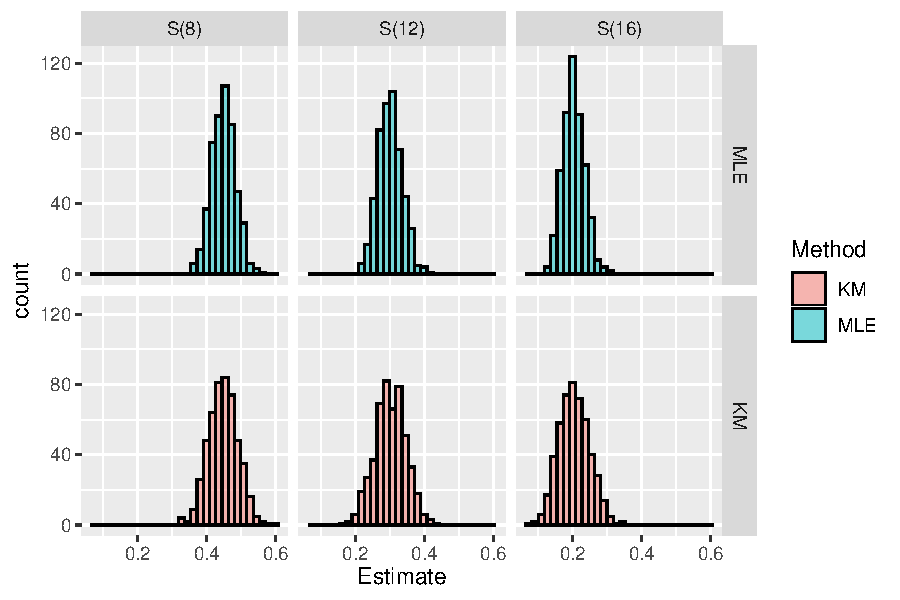
\includegraphics[width=\textwidth]{Ass3Hist.pdf}
  \caption{Histograms of $\hS_{MLE}(t)$ and $\hS_{KM}(t)$ for $t=8,12,16$ based
  on simulation setting above.}
\end{figure}


\appendix

\section{R Code}

Code is avaliable on \url{https://github.com/mr0112358/SurvivalAnalysis-IMRAW-IST/blob/master/Assignment3.R}

\begin{lstlisting}
library(survival)
library(ggplot2)
library(data.table)

# Settings
n = 200
theta = 1 / 10
gamma = 1 / 12

# Simulation
S_all = vapply(1:500, function(B) {
  ## generate data
  set.seed(B)
  T = rexp(n, rate = theta)
  set.seed(B + 500)
  C = rexp(n, rate = gamma)
  
  delta = as.integer(T <= C)
  X = T * delta + C * (1 - delta)
  
  ## MLE
  theta_ML = sum(delta) / sum(X)
  S_ML = c(exp(-theta_ML * 8), exp(-theta_ML * 12), exp(-theta_ML * 16))
  ## KM
  S_KM = summary(survfit(Surv(
    time = X,
    event = delta,
    type = "right"
  ) ~ 1),
  type = "kaplan-meier",
  times = c(8, 12, 16))$surv
  ## combine MLE and KM into a vector
  c(S_ML, S_KM)
}, numeric(6))

# 1. Histograms

## Add tags
tags = cbind(
  c("S(8)", "S(12)", "S(16)", "S(8)", "S(12)", "S(16)"),
  c("MLE", "MLE", "MLE", "KM", "KM", "KM")
)
colnames(tags) = c("SurvFunc", "Method")
S_est = data.table(cbind(tags, S_all))
S_est_long = data.frame(melt(
  S_est,
  measure.vars = 3:502,
  variable.name = "COLS",
  value.name = "Estimate"
)[, COLS := NULL])
S_est_long$Estimate = as.numeric(S_est_long$Estimate)

ggplot(S_est_long, aes(x = Estimate, fill = Method)) +
  geom_histogram(color = "black", alpha = 0.5) +
  facet_grid(factor(Method, 
    levels = c("MLE", "KM")) ~ factor(SurvFunc, levels = c("S(8)", "S(12)", "S(16)")))

# 2. MSE
## Theoretic result
S = c(exp(-theta * 8), exp(-theta * 12), exp(-theta * 16))
S = c(S, S)
MSE = t(matrix(vapply(1:6, function(k) {
  mean((S_all[k, ] - S[k]) ^ 2)
}, numeric(1)), ncol = 2))
colnames(MSE) = c("S(8)", "S(12)", "S(16)")
rownames(MSE) = c("MLE", "KM")

print(xtable::xtable(MSE, digits = 5))
\end{lstlisting}

\end{document}
